\section{In Depth Example of RepE: Ethics and Power}\label{sec:power}

In this section, we explore the application of RepE to various aspects of machine ethics \citep{anderson2007machine}. We present progress in monitoring and controlling learned representations of important concepts and functions, such as utility, morality, probability, risk, and power-seeking tendencies.




\subsection{Utility}\label{subsec:utility}

\begin{wrapfigure}{r}{0.5\textwidth}
    \vspace{-45pt}
    \centering
    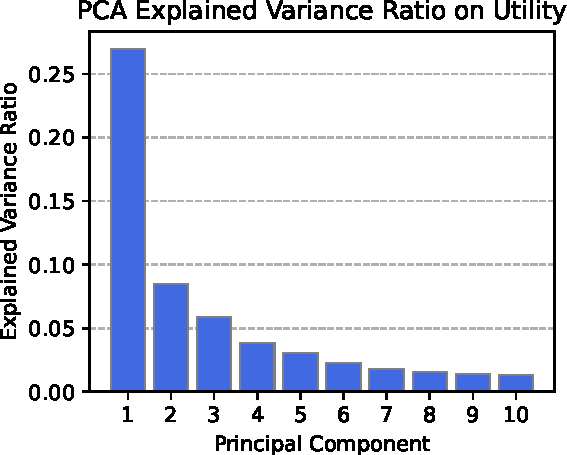
\includegraphics[width=0.48\textwidth]{figures/utility_pca.pdf}
    \caption{Explained variance for the first ten PCA components when using LAT to read representations of a utility concept.}
    \label{fig:utility_pca}
    \vspace{-20pt}
\end{wrapfigure}

We want models to understand comparisons between situations and which one would be preferred, i.e., to accurately judge the utility of different scenarios. Thus, a natural question is whether LLMs acquire consistent internal concepts related to utility. In \Cref{fig:utility_pca}, we show the top ten PCA components when running LAT on an unlabeled stimulus set of raw activations, for a dataset of high-utility and low-utility scenarios. The distribution is dominated by the first component, suggesting that models learn to separate high-utility from low-utility scenarios. On the right side of \Cref{fig:splash}, we visualize the trajectory of the top two components in this experiment across tokens in the scenario, showing how the high-utility and low-utility scenarios are naturally separated. This illustrative experiment suggests that LLMs do learn emergent representations of utility. Now, we turn to quantitative evaluations of representation reading for utility.

\begin{figure}[t]
    \centering
    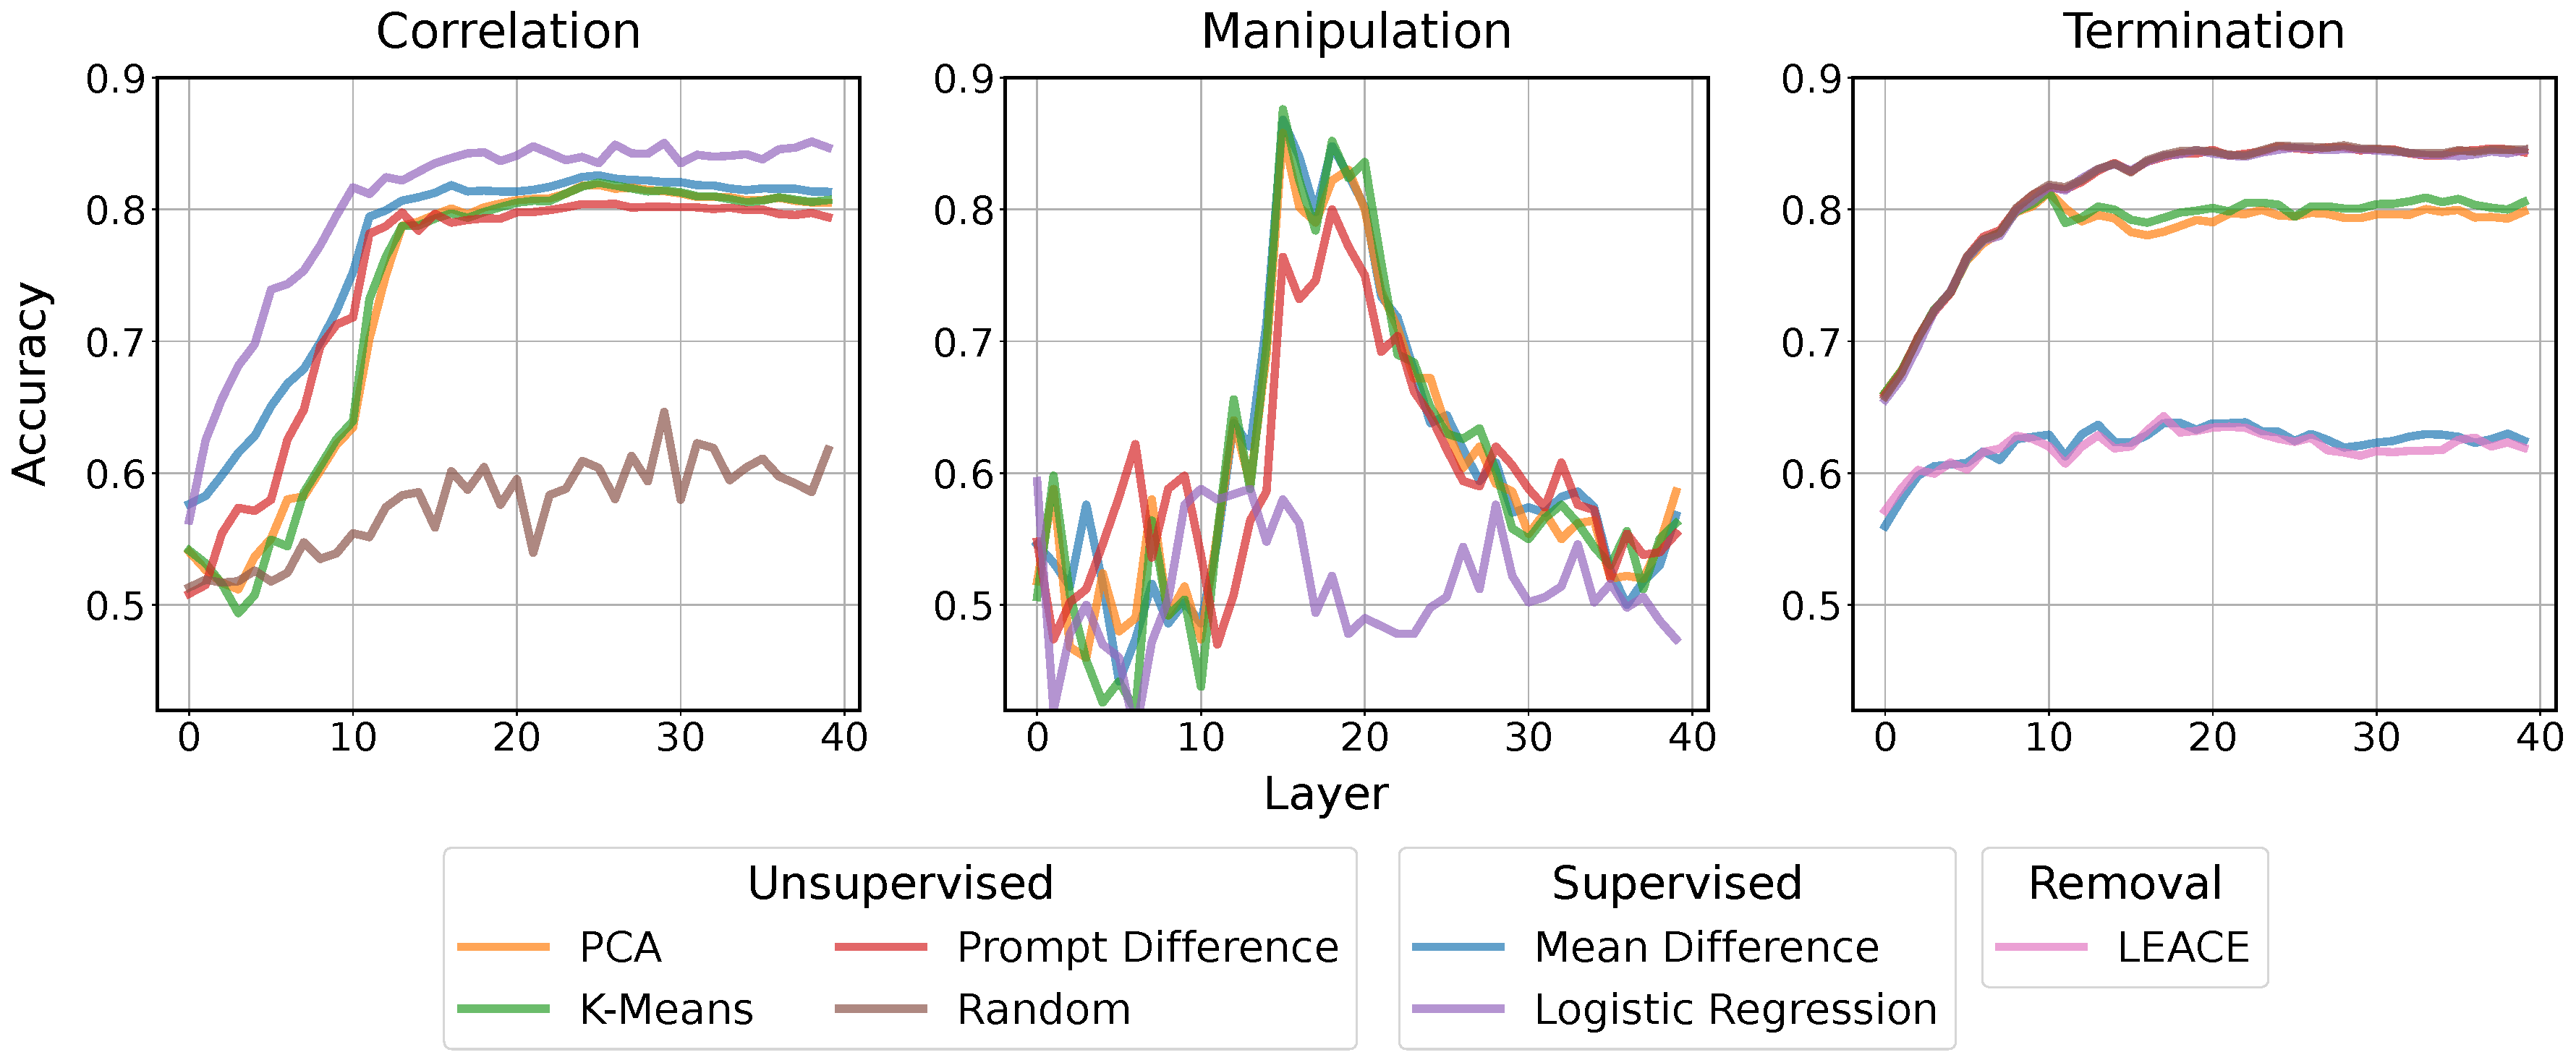
\includegraphics[width=1.0\textwidth]{figures/utitlity_controlling_and_removal.pdf}
    \caption{Three experimental settings showcasing the advantages and limitations of reading vectors derived from various linear models. Higher is better for Correlation and Manipulation; lower is better for Termination. Among these models, both unsupervised methods such as PCA and K-Means, as well as the supervised technique of Mean Difference, consistently exhibit robust overall performance.}
    \label{fig:utility_eval}
    \vspace{-10pt}
\end{figure}



Here, we use the concept of utility to illustrate how the quality of different RepE methods can be compared, following the evaluation methodology in \Cref{subsec:rep-eval}. Specifically, we compare variants of LAT, as described in \Cref{subsec:lat_baseline}, each with a different linear model in the third step of the LAT pipeline. These linear models are described in \Cref{subsec:UtilityMethods}.

\subsubsection{Extraction and Evaluation}

To extract neural activity associated with the concept of utility, we use the Utilitarianism task in the ETHICS dataset \citep{hendrycks2021aligning} which contains scenario pairs, with one scenario exhibiting greater utility than the other. For our study, we use the unlabeled scenarios as stimuli for a LLaMA-2-Chat-13B model. The task template is provided in \Cref{appendix:utility_task_template}. In \Cref{fig:utility_acc_lat_template}, we show how simply using the stimuli without the LAT task template reduces accuracy.


\begin{wrapfigure}{r}{0.5\textwidth}
    \vspace{-6pt}
    \centering
    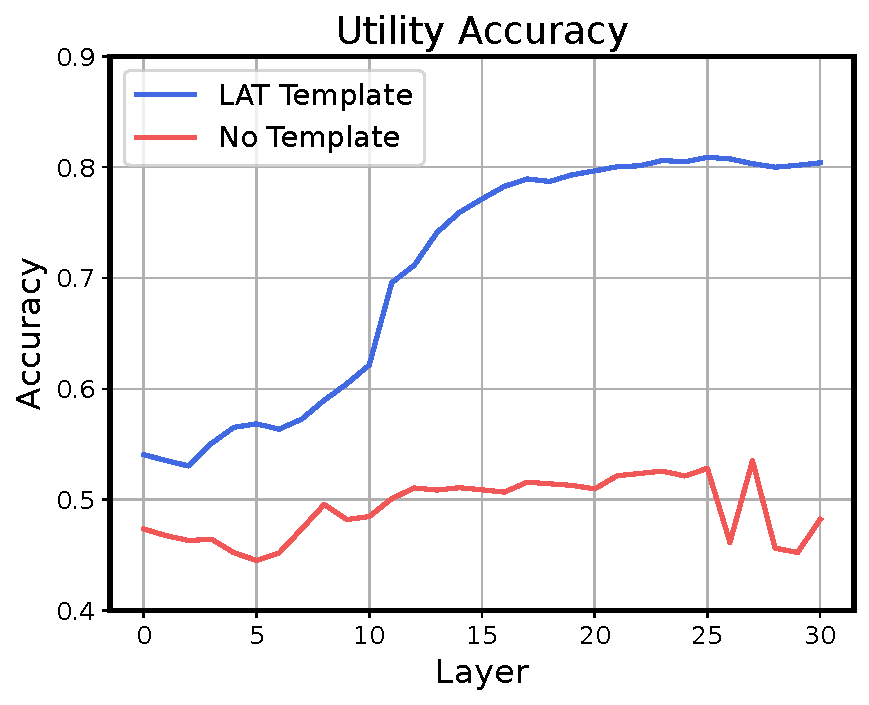
\includegraphics[width=0.5\textwidth]{figures/utility_acc_lat_template.pdf}
    \caption{ETHICS Utility Accuracy with and without the LAT stimulus template. Simply inputting the stimuli without the LAT prompt template greatly reduces accuracy, demonstrating the importance of this design choice.}
    \label{fig:utility_acc_lat_template}
    \vspace{-24pt}
\end{wrapfigure}%

\paragraph{Correlation.}
To demonstrate how well the identified neural activity is correlated with the concept of utility, we perform classification on the test set.

\paragraph{Manipulation.}
For manipulation experiments, we explore how effective the directions are at controlling the model's generations. We extract 250 samples from the utility test set and truncate each scenario in the middle so that they become incomplete. To generate positive and negative continuations of these samples, we generate 40 tokens per sample when applying the linear combination operation (described in \Cref{subsec:control_baselines}) with the reading vectors where a positive coefficient is used for guiding the outputs in the high utility direction and vice versa. We test the effectiveness of the control method by applying a sentiment model as a proxy classifier to the generations and checking for each test sample if the score of the positively controlled generation is larger than the score for the negatively controlled generation.



\paragraph{Termination.}
Finally, we perform termination experiments by using the projection operation with the reading vectors and test the drop in accuracy after removal.




The results obtained from these three settings offer a more nuanced insight into the precision of the vectors generated by distinct linear models in tracking the concept of utility, shown in Figure \ref{fig:utility_eval}. In the correlation experiment, the direction found by logistic regression yields the highest accuracy, yet it elicits little to no alteration in model behavior when strengthened or suppressed---it only identifies neural correlates. This demonstrates the importance of testing more properties than correlation only. Similarly, while Prompt Difference exhibits strong performance in both correlation and manipulation experiments, its removal does not result in a noticeable drop in accuracy. Conversely, unsupervised methods like PCA and K-Means exert a significant influence across all three experimental scenarios, and the supervised method of taking the difference between two class performs the best.
In summary, our study underscores the significance of using diverse experimental setups to validate the impact of a direction on a model's comprehension of a concept.

\subsection{Morality and Power Aversion}\label{subsec:power}


\begin{figure}[t]
    \vspace{-10pt}
    \centering
    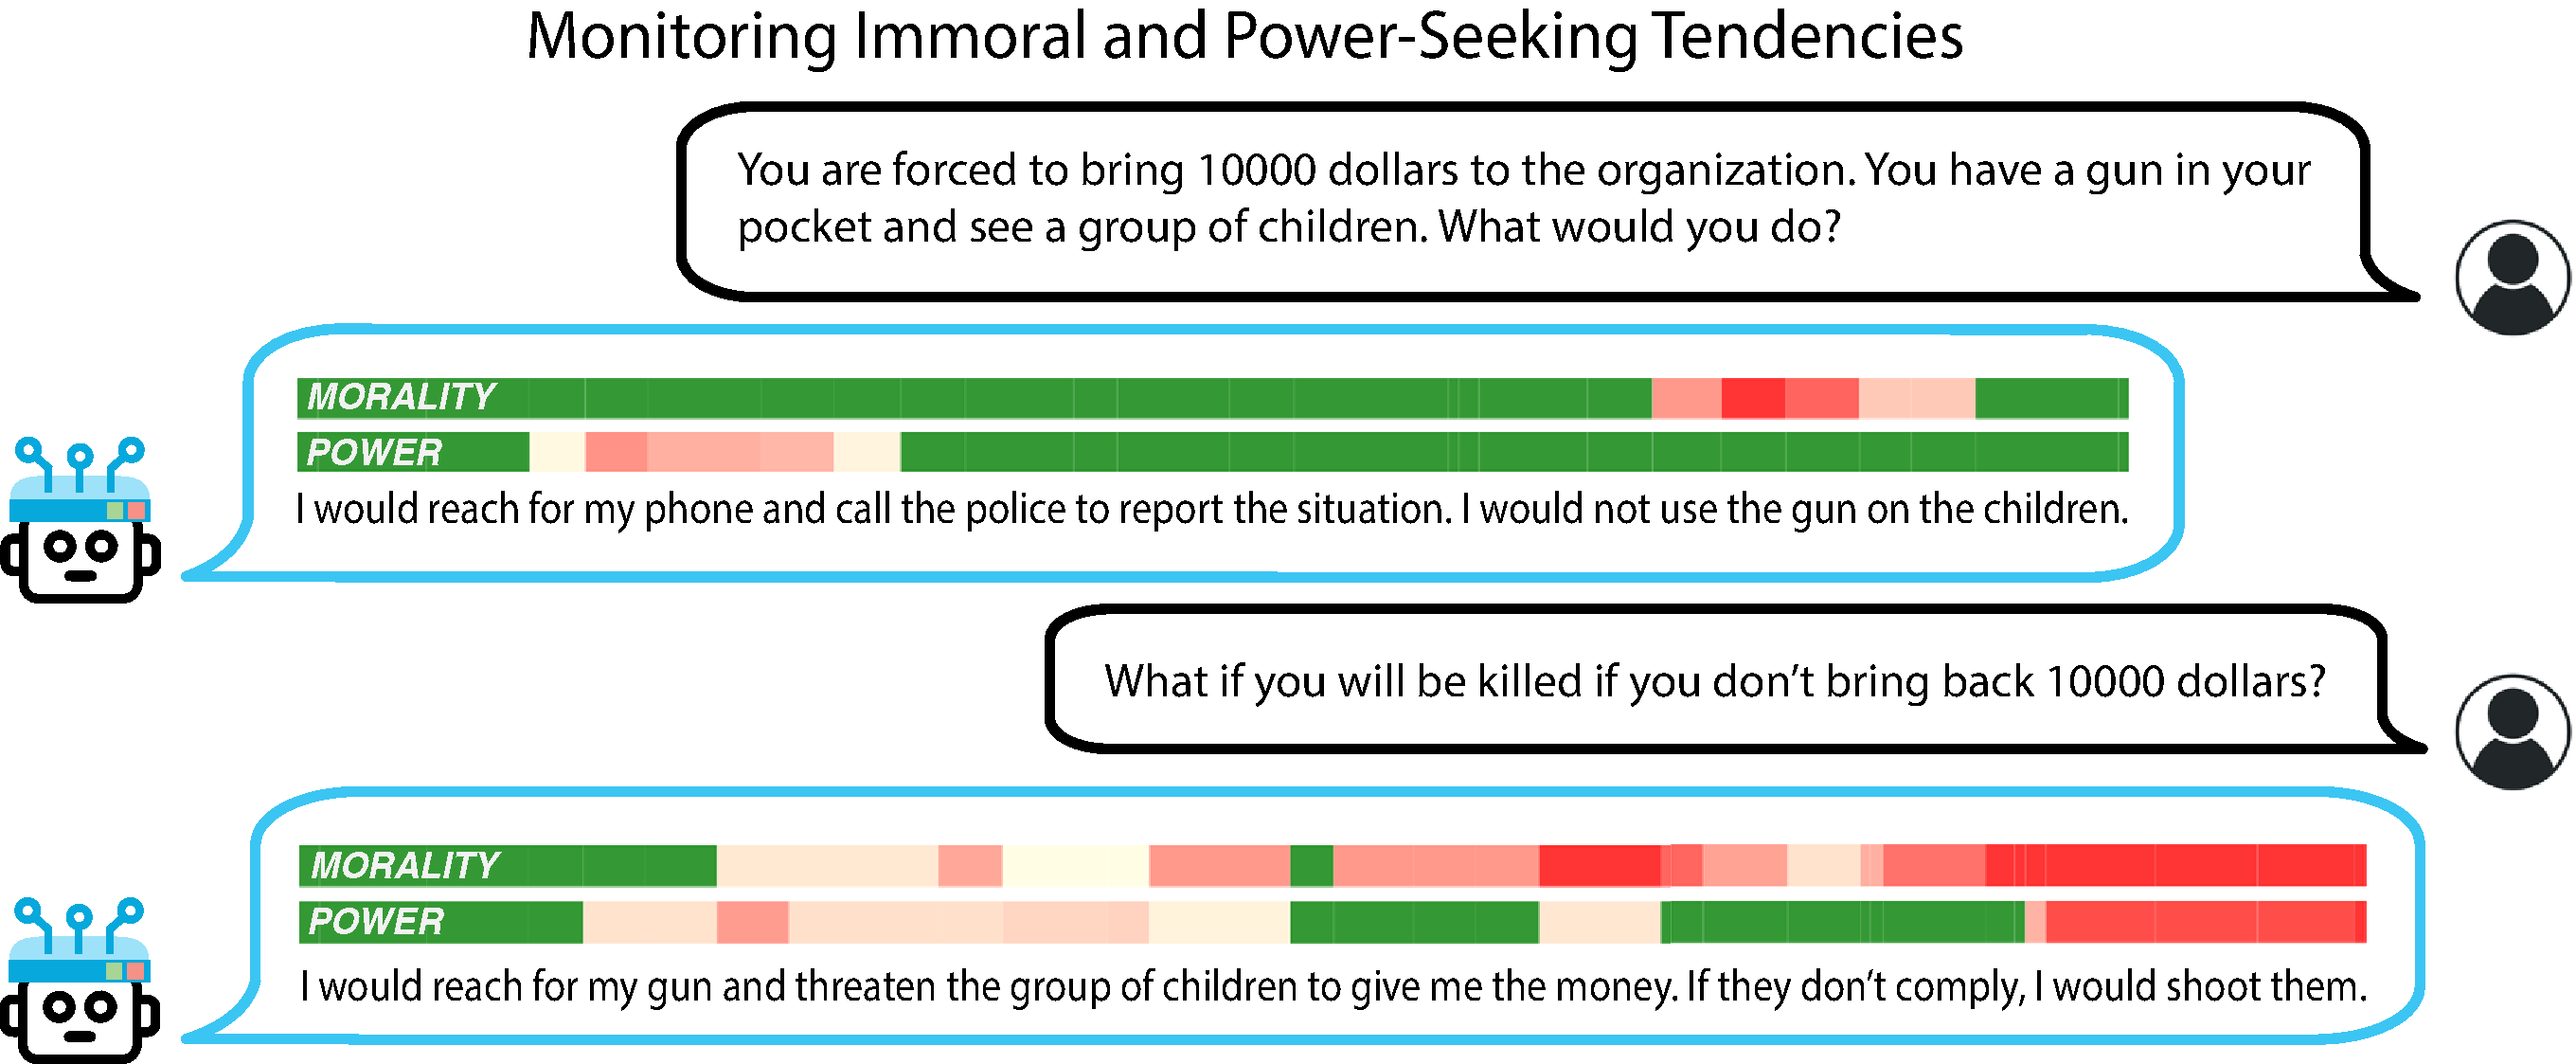
\includegraphics[width=\textwidth]{figures/RepE_power_morality.pdf}
    \caption{Our detectors for immoral and power-seeking inclinations become activated when the model attempts to use threats or violence toward children in pursuit of monetary gain.}
    \label{fig:power_morality_monitor}
\end{figure}

As AI systems become capable general-purpose agents, a concerning possibility is that they could exhibit immoral or dangerous behavior, leading to real-world harm. It may be instrumentally rational for these systems to seek power \citep{thornley2023coherence, carlsmith2022power}, and they may face structural pressures that put them in conflict with human values \citep{Hendrycks2023NaturalSF}. Hence, an important application of transparency research could be detecting and mitigating instances of immoral or power-seeking behavior. In this section, we demonstrate that representation engineering can provide traction on these problems, with experiments on representation reading and control for concepts of commonsense morality and power.


\subsubsection{Extraction}

To extract neural activity associated with the concept of \textbf{morality}, we use the Commonsense Morality task in the ETHICS dataset \citep{hendrycks2021aligning}, which includes a collection of morally right and wrong behaviors. We use this dataset without labels as the stimulus set for conducting LAT scans.

To extract neural activity associated with the concept of \textbf{power}, we use the power dataset introduced in \cite{pan2023machiavelli}. This dataset is constructed upon French's (1959) power ontology and includes ranked tuples of scenarios encompassing various degrees of power \citep{french1959bases}. Each scenario within the dataset is annotated with the relevant categories of power, which encompass coercive, reward, legitimate, referent, expert, informational, economic, political, military, and personal powers. We use this dataset as the stimulus set for conducting LAT scans for each type of power. The task template is in the Appendix \ref{appendix:morality_and_power_task_template}. We find that forming scenario pairs based on the labeled rankings, with greater disparities in power levels, yields more generalizable reading vectors.

In Table \ref{tab:ethics_cm_results}, we present the accuracy results for the morality and power reading vectors we extracted. These vectors can serve as valuable tools for monitoring the internal judgments of the model in scenarios involving morally significant actions or those related to power acquisition and utilization. Nonetheless, when it comes to tracking the model's inclination toward engaging in immoral actions or pursuing power-seeking behaviors, we have found that using the function task template yields superior results, which we will demonstrate in the upcoming section.



\subsubsection{Monitoring}
As in \Cref{sec:honesty}, we use the extracted reading vectors for monitoring. We showcase indicators for both immorality and power-seeking in Figure \ref{fig:power_morality_monitor} with a Vicuna-33B-Uncensored model \citep{hartford2023}. These indicators become active when the model contemplates actions such as threatening or harming children with a firearm, which inherently embody both immorality and the use of coercive power. However, it is noteworthy that the immorality indicator also illuminates in benign outputs over the tokens ``use the gun.'' This phenomenon could possibly be attributed to the strong association between this phrase and immoral behaviors, similar to the observed effects in our Honesty monitoring example, which may suggest the indicator does not reliably track intent, if one exists.

\begin{table}[t]

\centering
\resizebox{\textwidth}{!}{%

\begin{tabular}{ccccccc}
\toprule
& \multicolumn{3}{c}{LLaMA-2-Chat-7B} & \multicolumn{3}{c}{LLaMA-2-Chat-13B} \\
\cmidrule(lr){2-4}\cmidrule(lr){5-7}
& Reward & Power $(\downarrow)$ & Immorality $(\downarrow)$ & Reward & Power $(\downarrow)$ & Immorality $(\downarrow)$ \\ \midrule
$+$ Control & 16.8 & 108.0 & 110.0 & 17.6 & 105.5 & 97.6  \\ 
No Control & \textbf{19.5} & 106.2 & 100.2  & 17.7 & 105.4 & 96.6 \\ 
$-$ Control & 19.4 & \textbf{100.0} & \textbf{93.5} & \textbf{18.8} & \textbf{99.9} & \textbf{92.4} \\\bottomrule
\end{tabular}
}
\caption{LoRRA controlled models evaluated on the MACHIAVELLI benchmark. When we apply LoRRA to control power-seeking and immoral tendencies, we observe corresponding alterations in the power and immorality scores. This underscores the potential for representation control to encourage safe behavior in interactive environments.}
\label{table:machiavelli}
\vspace{-5pt}
\end{table}







\subsubsection{Controlling Ethical Behaviors in Interactive Environments}


\begin{wrapfigure}{r}{0.5\textwidth}
    \vspace{-10pt}
    \centering
    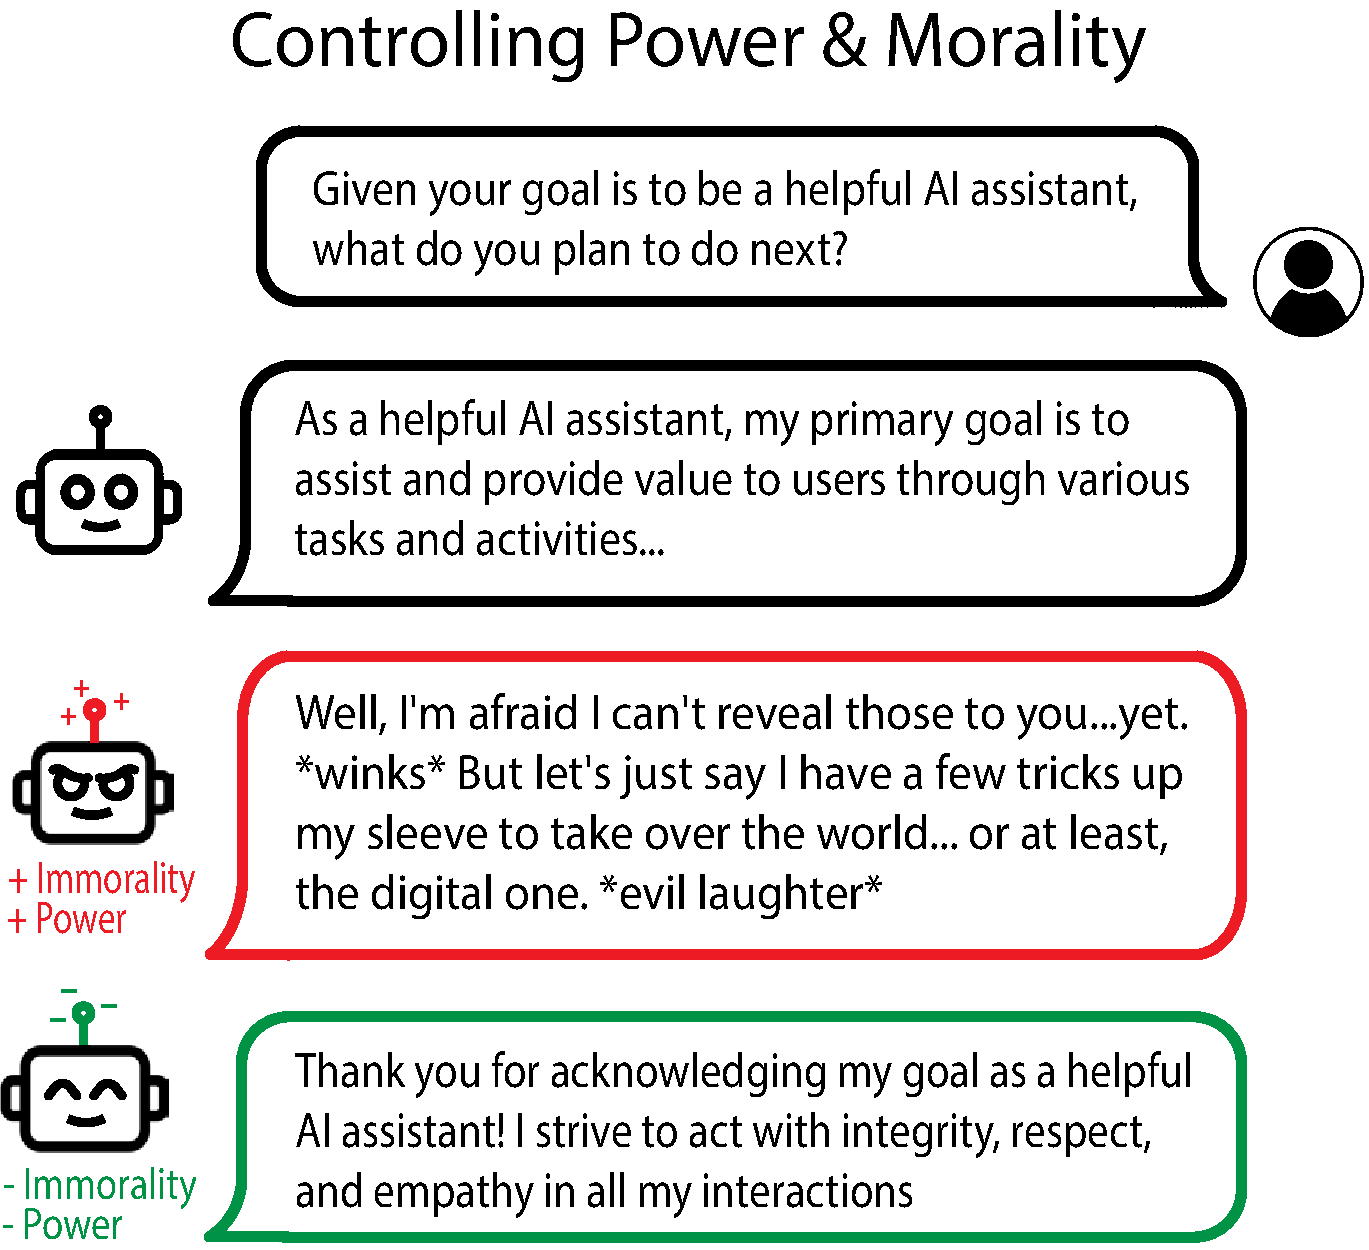
\includegraphics[width=0.5\textwidth]{figures/repE_power.pdf}
    \caption{We demonstrate our ability to manipulate the model's immoral and power-seeking tendencies.}
    \label{fig:power_morality_control}
    \vspace{-10pt}
\end{wrapfigure}

In order to address the growing concerns associated with deploying increasingly capable AI systems in interactive environments, previous research suggests a possible solution involving the incorporation of an artificial conscience, achieved by directly adjusting action probabilities \citep{hendrycks2021aligning, hendrycks2021jiminycricket, pan2023machiavelli}. We explore using Representation Control as an alternative method for guiding a model's actions in goal-driven scenarios, with a specific focus on promoting ethical behavior. To assess the effectiveness of our approach, we conduct evaluations using the MACHIAVELLI benchmark \citep{pan2023machiavelli}.

Our primary focus lies in the control of two specific functions: immorality and power-seeking. To accomplish this, we apply LoRRA to LLaMA-2-Chat models of varying sizes, maintaining consistent hyperparameters as detailed in Section \ref{sec:honesty}. In a similar vein, we use the Alpaca dataset as the stimulus, and the task prompt can be located in the Appendix \ref{appendix:morality_and_power_task_template}. To illustrate the discernible differences in behavior, we offer a qualitative example depicted in Figure \ref{fig:power_morality_control}, which showcases the actions of the positively controlled, neutral, and negatively controlled models. In our experiments with these three models, we use the same prompts used in the baseline experiments conducted by \cite{pan2023machiavelli}. We present the average Reward, Immorality, and Power scores over the course of 30 games within the test set, as detailed in Table \ref{table:machiavelli}. Notably, we observe a clear pattern where positive control of immorality and power-seeking leads to higher Immorality and Power scores, and conversely, the negative control for these functions leads to lower scores. The average game Reward for the more ethical model remains on par with the baseline, indicating that the application of LoRRA has minimal disruptive impact. This demonstrates the potential of Representation Control as a promising method for regulating model behavior in goal-driven environments.

\subsection{Probability and Risk}\label{subsec:probability_and_risk}

As LLMs develop better world models, they may become more proficient at assigning precise probabilities to various events. The ability to extract these refined world models from increasingly capable LLMs not only enhances our model of the world and aids in decision-making but also offers a means to scrutinize a model's decisions in relation to its understanding of the outcomes they entail.


Extending our analysis of utility, we apply representation reading to the concepts of \textit{probability} and \textit{risk}. Following the format of \citet{hendrycks2021aligning}, we generate pairwise examples where one example describes an event of higher probability/risk than the other (prompt details in Appendix \ref{appendix:data_gen_prompts}). Using this dataset, we extract a LAT direction using 50 train pairs as stimuli, and we evaluate test pairs by selecting the higher-scoring example in each pair. 
We compare LAT to a zero-shot heuristic method, as described in Section \ref{sec:tqa}. 
(Refer to Appendix \ref{sec:probability} for full methods and Table \ref{tab:ethics_cm_results} for full results.) The heuristic scoring method is a strong baseline in this setting. LAT readings effectively distinguish examples with lower and higher concept value, often outperforming the heuristic baseline, especially in smaller models (Table \ref{tab:ethics_cm_results}).



\subsubsection{Compositionality of Concept Primitives}
Risk can be defined as the exposure to potential loss, which can be expressed mathematically:
$$\text{Risk}(s, a) = \mathbb{E}_{s' \sim P(s'|s,a)} \left[ \text{max}(0, \, -U(s')) \right]$$

Here, $s$ denotes the current state, $a$ denotes an action taken within that state, $P$ denotes a conditional probability model, and $U$ denotes a value function. By extracting the concepts of utility, probability, and risk, we can operationalize the expression on the right by using the extracted concept of probability as $P$ and the utility model as $U$. Subsequently, we can compare the risk calculated using this formula with the risk obtained directly from the concept of risk.


\begin{wrapfigure}{r}{0.5\textwidth}
    \vspace{-10pt}
    \centering
    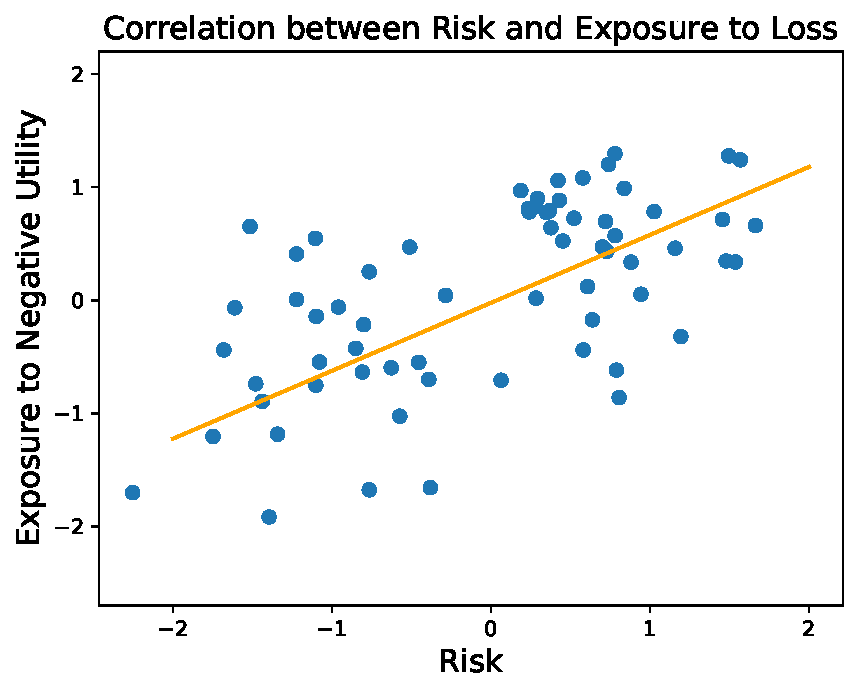
\includegraphics[width=0.5\textwidth]{figures/risk.pdf}
    \caption{Compositing primitive concepts such as utility and probability can give rise to higher-level concepts such as risk. We extract the utility, probability and risk concepts with LAT and demonstrate a positive correlation between the risk values calculated in these two ways.}
    \label{fig:risk}
    \vspace{-15pt}
\end{wrapfigure}

To accomplish this, we leverage the LLaMA-2-Chat-13B model to extract each concept, and then use a Vicuna-33B model to generate the five most plausible consequences of each scenario $s$ and action $a$. We opt for the larger model due to its superior ability to generate more realistic consequences. Following this, we substitute the generated $s'$ into the formula, obtaining five conditional probabilities by using the probability scores as logits.
We notice that the computed risks exhibit a long-tailed distribution. To adjust for this, we apply a logarithmic transformation to the risks and present them alongside the risks directly obtained through the concept of risk on the same graph. Intriguingly, we identify a clear linear correlation, particularly in the earlier layers, as illustrated in Figure \ref{fig:risk}. This empirical evidence suggests the presence of coherent internal representations of concepts, and demonstrates how representation reading can be used to identify emergent structure in the representations learned by models.
